% Created 2026-09-03 Thu 16:43
% Intended LaTeX compiler: pdflatex
\documentclass[doc]{apa7}
                 \usepackage[american]{babel}

\authorsnames[1, 1]{Jinghui Liang, Dale J. Barr$^*$}
\authorsaffiliations{{School of Psychology and Neuroscience, University of Glasgow, UK}}
\leftheader{Supplementary Materials, Liang \& Barr}
\shorttitle{Supplementary Materials, Liang \& Barr}
\usepackage{parskip}
\keywords{experimental design, statistical power, measurement}
\authornote{$^*$Corresponding author: Dale J. Barr, School of Psychology \& Neuroscience, University of Glasgow, 62 Hillhead Street, Glasgow, UK, G12 8QB. Email: dale.barr@glasgow.ac.uk.}
\usepackage{longtable}
\usepackage{soul}
\hypersetup{colorlinks,citecolor=blue,linkcolor=blue,urlcolor=red}
\date{\today}
\title{Supplementary materials for Liang and Barr, ``Improving power without increasing sample size''}
\hypersetup{
 pdfauthor={Dale},
 pdftitle={Supplementary materials for Liang and Barr, ``Improving power without increasing sample size''},
 pdfkeywords={},
 pdfsubject={},
 pdfcreator={Emacs 29.3 (Org mode 9.6.15)}, 
 pdflang={English}}
\makeatletter
\newcommand{\citeprocitem}[2]{\hyper@linkstart{cite}{citeproc_bib_item_#1}#2\hyper@linkend}
\makeatother

\usepackage[notquote]{hanging}
\begin{document}

\maketitle

\section*{Supplementary simulations}
\label{sec:orgd7f958c}

\setlength{\parindent}{0cm}

We undertook a set up supplementary simulations to find optimal parameters for Wiggly Intercept Models (WIMs) given the independent variables of error structure, number of levels of the independent variable, and number of repetitions. The latter of these three variables determines the number of trials in the experiment.

In the first subsection, we describe simulations that we rand to determine the best type of basis function to use, comparing the default ``thin plate'' (\texttt{tp} option) to cubic regression (\texttt{cr} option) and P-splines (\texttt{ps} option). This suggested that P-splines performed best for improving power, although differences were very small.

In the second subsection, we describe simulations to determine the optimal number of basis function for each combination of type of error structure, number of levels, and number of repetitions.

\subsection*{1. Type of basis function}
\label{sec:orgff789e3}

Because running simulations for the full set of parameter values would be take too much time, we focused on a single set of parameters for a medium sized design (\texttt{4} levels and \texttt{12} repetitions, or \texttt{48} trials), under the assumption that any advantages seen here would hold for other types of designs.

The number of participants for each dataset was \texttt{40}, which differs from the number in the paper (25) because these simulations were run as part of an earlier version of the project. We see no reason for concern that these results would diverge for a smaller number of participants; in any event, the results are fairly similar across the different types of basis functions, making the choice somewhat arbitrary. Model syntax was as described in the main paper. 

\begin{figure}[htbp]
\centering
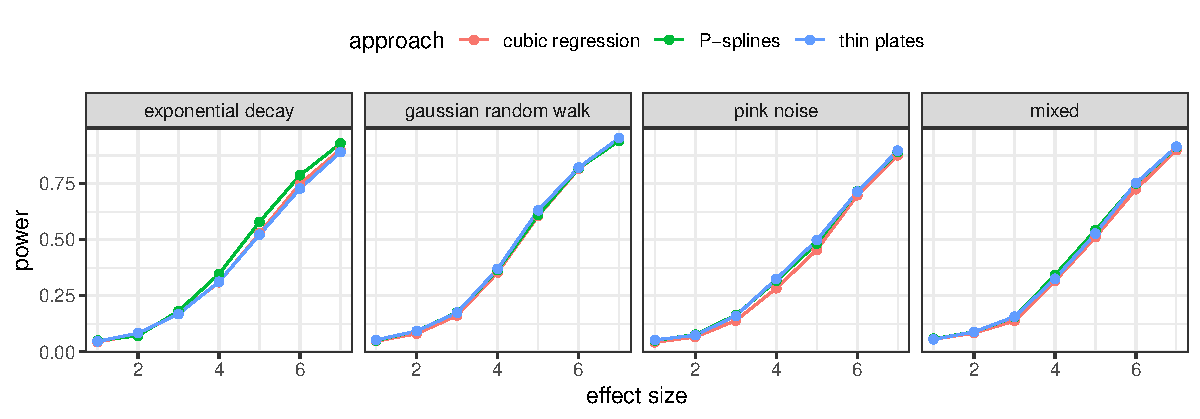
\includegraphics[width=.9\linewidth]{fig/compare-basis.pdf}
\caption{\label{fig:orge392dd9}Power for the three basis function types by effect size and error structure.}
\end{figure}

Figure~\ref{fig:orge392dd9} shows the results for \texttt{755} simulations at each setting of error structure and effect size. Differences are minor, but p-splines show the best performance numerically, evident mainly for the exponential decay setting.

\subsection*{2. Number of basis functions}
\label{sec:orge32cc41}

We fixed the basis function to be P-splines and the number of participants to be 25, and ran a set of simulations to determine the optimal number of basis functions for each type of dataset, given the error structure, number of levels of the within factor, and number of repetitions per level. The minimum number of allowed basis functions was 6; the maximum was 1/3 of the number of trials (which as one of 12, 24, 48, 96, or 192, depending on the number of levels and number of repetitions). In these simulations, we set the \texttt{k} parameter of the factor smooth to the maximum, and then extracted the ``estimated degrees of freedom'' (edf) to see if a smaller value was admissible. We ran at least 200 simulations at each of the \texttt{36} parameter settings obtained by combining the four error structures, the three numbers of levels of the IV, and the three numbers of repetitions. We calculated the mean edf at each parameter setting and used that as our value, unless it was less than six, in which case six basis functions were used.

\begin{figure}[htbp]
\centering

\includegraphics[width=.9\linewidth]{fig/n-basis.pdf}
\caption{\label{fig:orgcb8b31f}Optimized number of basis functions for WIMs derived from 200 simulations runs for each type of error structure, levels of the independent variable, and number of repetitions. The dashed line in the background represents the maximum allowed number, either 1/3 of the number of trials or six, whichever is bigger.}
\end{figure}

The selected number of basis functions are shown in Figure~\ref{fig:orgcb8b31f}. 
\end{document}
